
\documentclass[aspectratio=169,11pt]{beamer}
% customize block aesthetics
\definecolor{customblue}{rgb}{0.13,0.28,0.59}
\setbeamercolor{block title}{bg=customblue, fg=white}
\setbeamercolor{block body}{bg=customblue!10}
\setbeamertemplate{blocks}[rounded]
\usepackage{array,color,graphicx,comment,tikz}
\usepackage{bibentry,amsmath,verbatim}
\bibliographystyle{abbrv}
\setbeamertemplate{bibliography entry title}{}
\setbeamertemplate{bibliography entry location}{}
\setbeamertemplate{bibliography entry note}{}
\setbeamercolor{bibliography entry author}{fg=black}
\setbeamercolor{bibliography entry title}{fg=gray}
%\usetikzlibrary{calc,patterns,decorations.pathmorphing,decorations.markings}
\input talk_defs.tex
%\input formatting.tex

\mode<presentation>
{
\usetheme{default}
}

\setbeamertemplate{navigation symbols}{}
\usecolortheme[rgb={0.13,0.28,0.59}]{structure}
\setbeamertemplate{itemize subitem}{--}
\newcommand\footlineon{
\setbeamertemplate{footline} {
\begin{beamercolorbox}[ht=2.5ex,dp=1.125ex,leftskip=.8cm,rightskip=.6cm]{structure}
%\footnotesize \insertsection
\hfill
{\insertframenumber}
\end{beamercolorbox}
\vskip 0.45cm
}
}
\footlineon

\AtBeginSection[] 
{ 
	\begin{frame}<beamer> 
		\frametitle{Outline} 
		\tableofcontents[currentsection,currentsubsection] 
	\end{frame} 
}
\usepackage{listings}
%%% Custom listing format
\definecolor{seagreen}{rgb}{0.18, 0.55, 0.34}
\definecolor{mediumviolet-red}{rgb}{0.78, 0.08, 0.52}
\definecolor{khaki}{rgb}{0.94, 0.9, 0.55}
\definecolor{background-gray}{gray}{0.95}
\setbeamertemplate{footline}{
  \hfill 
  \usebeamerfont{page number in head/foot}
  \usebeamercolor[fg]{page number in head/foot}
  \small 
  \insertframenumber \hspace*{2ex} \vspace*{2ex} 
}

\lstdefinelanguage{mypython}
{
keywords=[1]{from, import, as, assert, not, print, nonneg, PSD, qcp, pos, axis,
             for, in, bool},
keywordstyle=[1]{\color{mediumviolet-red}},
keywords=[2]{surecr, torch, cp, lo, pl, cvxpy, dsp, Variable, LocalVariable,
        sqrt, exp, saddle_inner, saddle_max, saddle_min, SaddlePointProblem, MinimizeMaximize,
        numpy, np, Problem, Minimize, Maximize, is_dsp, solve, inner,
        convex_variables, concave_variables, affine_variables, sum, mean, multiply,
        triu, astype, reshape,
        arange, range, norm1, norm2, norm_inf, abs, square, saddle_quad_form, norm,
        sum_values, sum_squares, inv_pos, huber, diff, log, log_sum_exp, Parameter,
        append, ones, diag, np, power, ppf, quad_over_lin, cholesky,
        diagonal, outer, array, linalg, inv, log_det, quad_form, status, hstack},
keywordstyle=[2]{\color{seagreen}},
upquote=true,
showstringspaces=false,
basicstyle=\ttfamily\small,
columns=fullflexible,
keepspaces=true,
emph={True,False,def,return,float,class,match,switch,len},
emphstyle={\color{seagreen}},
backgroundcolor = \color{background-gray},
belowskip=1em,
aboveskip=1em,
morecomment=[l]{\#}
}
%% begin presentation
\title{
REGROW: Renewable Energy Generation Risk from Outlier Weather
}

\author{
\textbf{Giray Ogut}\inst{1} \and 
Bennet Meyers\inst{2} \and
David Chassin\inst{2} \and
Kirsten Perry\inst{3} \and
Stephen Boyd\inst{1} \and
}

\institute{
\inst{1} Stanford University \\
\inst{2} SLAC National Accelerator Laboratory \\
\inst{3} National Renewable Energy Laboratory
}

\date{\small Cybersecurity and Technology Innovation Conference, 7/31/2024}

\begin{document}

\begin{frame}
\titlepage
\end{frame}

\begin{frame}{Overview}
\BIT
\item \textbf{motivation:} 2020 CAISO blackouts caused by \\
\hspace{12mm} $-$ extreme weather: very high energy demand \\
\hspace{12mm} $-$ high renewable penetration: `duck curve' effect\\
\hspace{12mm} $-$ day-ahead electricity market: supply challenges\\
\item \textbf{objectives:} \\
\hspace{12mm} $-$ estimation of correlated losses and fat tails \\
\hspace{12mm} $-$ robust model predictive control of the grid \\
\hspace{12mm} $-$ counterfactual reasoning for different scenarios\\
\item \textbf{model:} white-box ML model based on convex optimization for \\
\hspace{12mm} $-$ joint probability distribution of load and renewable generators \\
\hspace{12mm} $-$ efficient, tractable and robust planning
\EIT
\end{frame}

\begin{frame}{Dataset curation and grid modeling}
\begin{columns}
	\begin{column}{0.42\textwidth}
		\begin{figure}
			\centering
			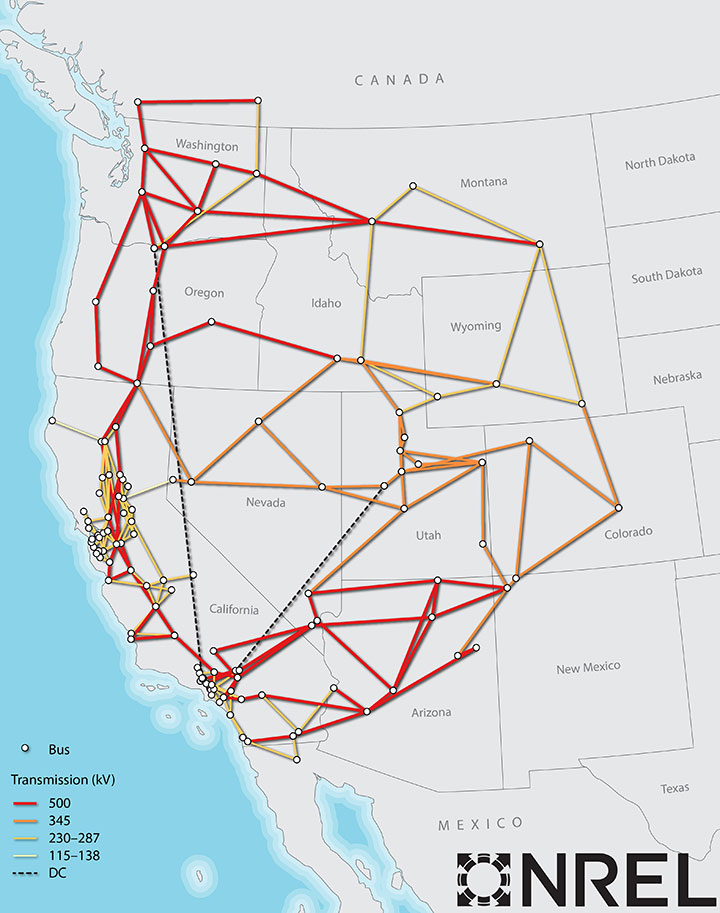
\includegraphics[width=\columnwidth]{./figures/weccmap.jpg}
		\end{figure}
	\end{column}
	\begin{column}{0.58\textwidth}
		\BIT
		\item curate datasets covering historical abnormal weather patterns
		\item obtain multidimensional data covering grid conditions, renewable generation, and weather
		\item \textbf{example datasets} \\
		\hspace{12mm} $-$ NREL PVFleets \\
		\hspace{12mm} $-$ NREL 144-bus model of WECC electrical grid\\
		\hspace{12mm} $-$ NOAA extreme weather\\
		\EIT
	\end{column}
\end{columns}
\end{frame}

\begin{frame}{Risk modeling}
\begin{columns}
	\begin{column}{0.55\textwidth}
		\begin{figure}
			\centering
			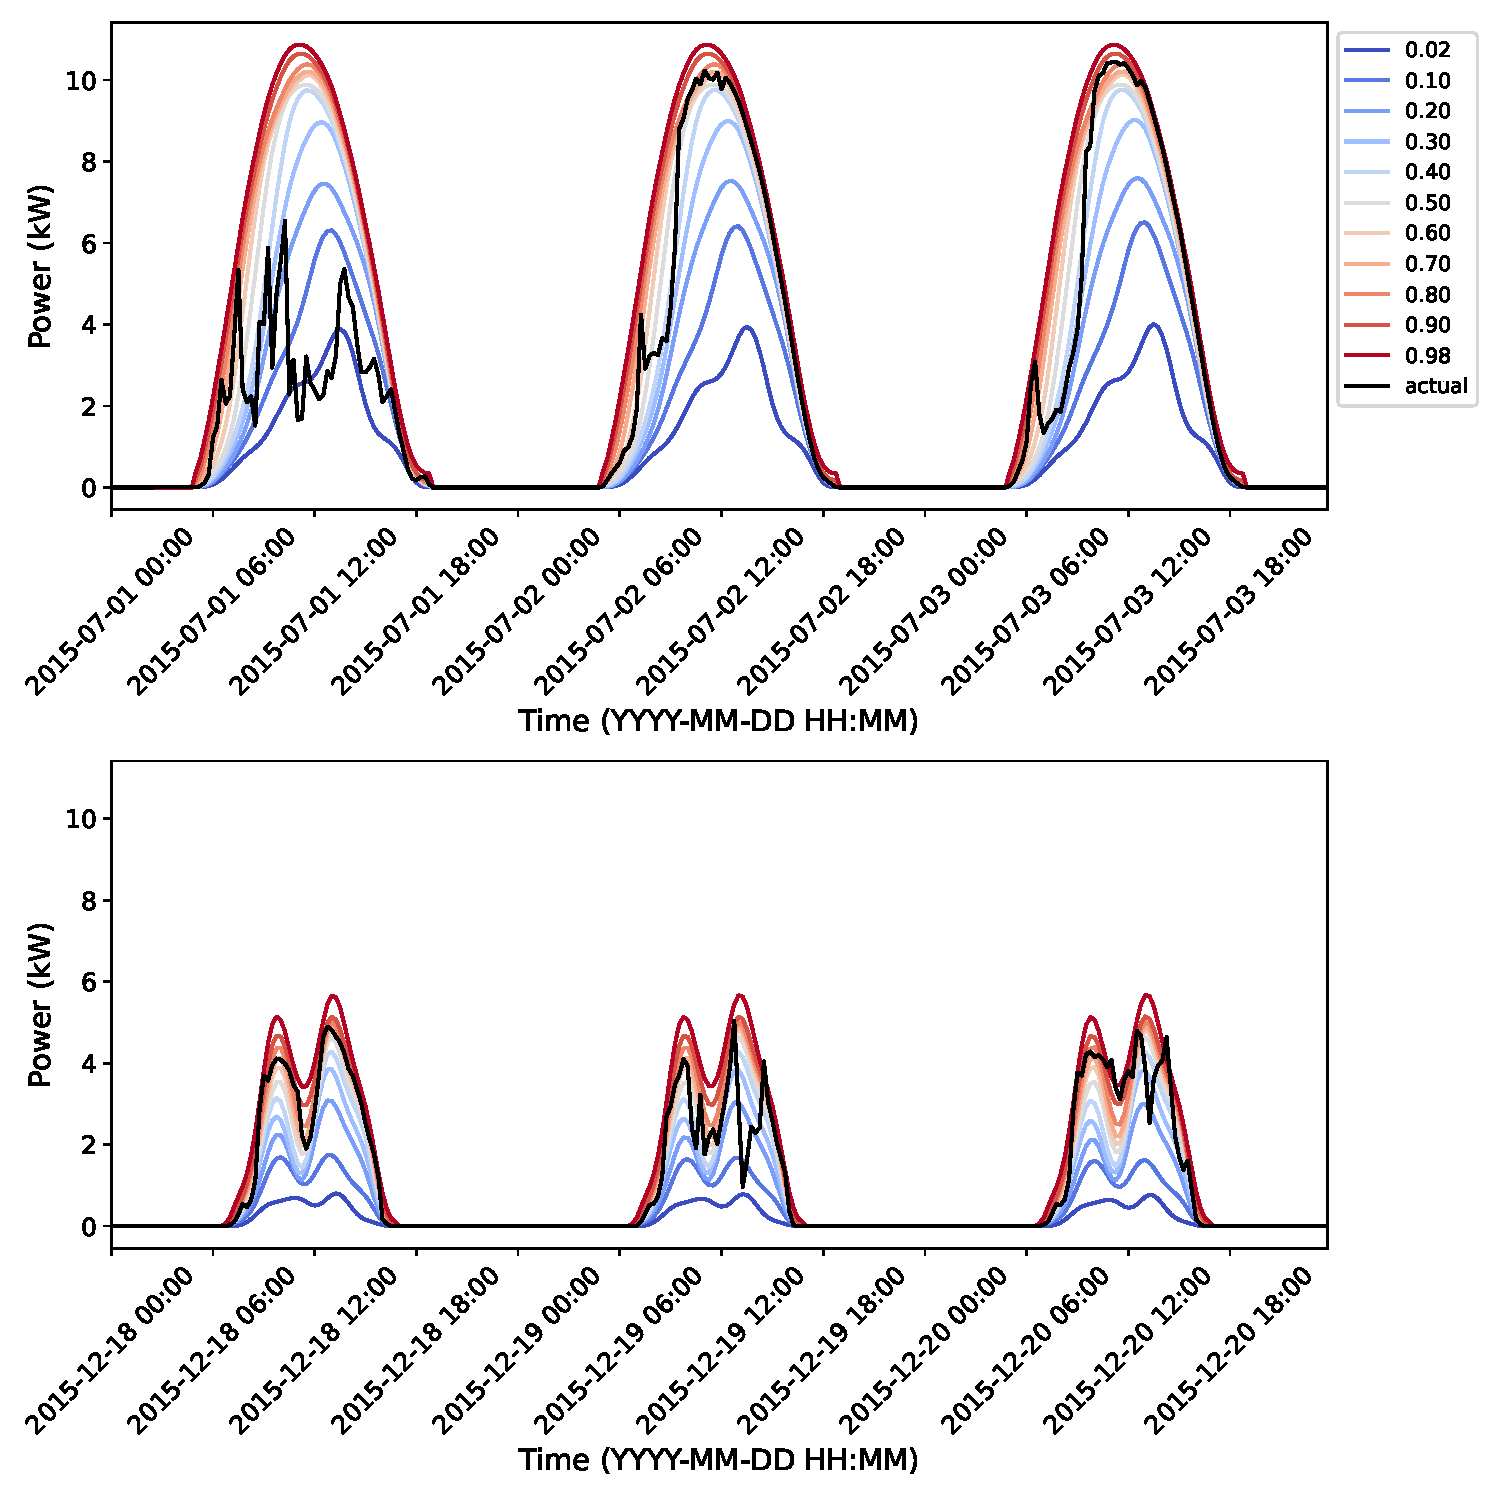
\includegraphics[width=\columnwidth]{./figures/quantiles_mapped_back.pdf}
		\end{figure}
	\end{column}
	\begin{column}{0.45\textwidth}
		\BIT
		\item develop risk models of renewable generator underperformance and outages
		\item capture correlations between generators and ambient meteorological conditions
		\item make a `nightmare scenario generator'
		\item figure shows estimated quantiles for power generation of a residential PV system
		\EIT
	\end{column}
\end{columns}
\end{frame}

\begin{frame}{Robust control}
\BIT
\item model predictive control (MPC) consisting of \\
\hspace{12mm} $-$ \textbf{forecast:} predict stochastic future values \\
\hspace{12mm} $-$ \textbf{plan:} solve optimization problem assuming forecasts are correct \\
\hspace{12mm} $-$ \textbf{execute:} take first action in plan \\
\hspace{12mm} $-$ \textbf{repeat} 
\item works extremely well in practice (\eg \ to land rockets)
\item can be specified as a convex optimization problem
\item tractable and can be solved efficiently and robustly
\EIT
\end{frame}

\begin{frame}{Multi-forecast MPC}
\begin{columns}
	\begin{column}{0.65\textwidth}
		\begin{figure}
			\centering
			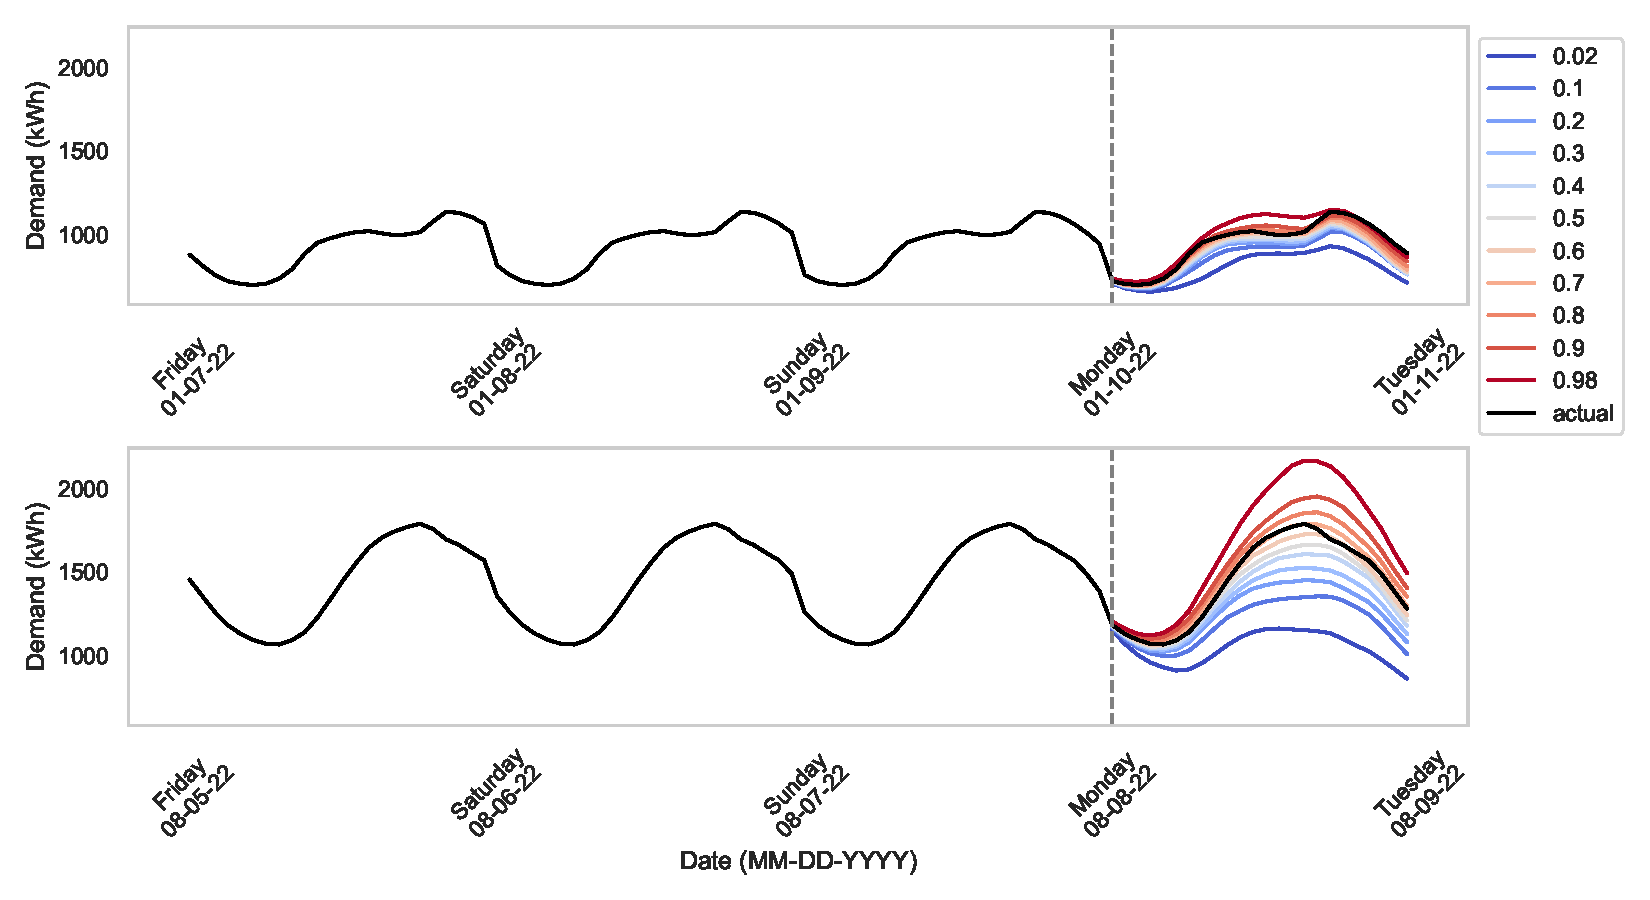
\includegraphics[width=\columnwidth]{./figures/marginal_quantile_forecasts.pdf}
		\end{figure}
	\end{column}
	\begin{column}{0.35\textwidth}
		\BIT
		\item incorporate uncertainty and information patterns via multiple scenarios
		\item can be conditioned on historical and future information 
		\item figure shows net load forecast for Rhode Island
		\EIT
	\end{column}
\end{columns}
\end{frame}

\begin{frame}[fragile]{Implementation}
\begin{columns}
	\begin{column}{0.45\textwidth}
		
\[
	\begin{array}{ll}
		\mbox{minimize}   &  -q_T + \kappa \| c \|_1 + \sum_{t=1}^{T}\phi(g_t) \\
		\mbox{subject to} & q_1 = Q^{\mbox{init}}, \\
		& q_{t+1} = q_t + c_t, t = 1, \ldots, T, \\
		& 0 \preceq r^{\mbox{curt}} \preceq r, \\
		& c + r^{\mbox{curt}} + g = l, \\
		& 0 \preceq q \preceq Q \ones, \\
		& 0 \preceq g \preceq G \ones, \\
		& |c| \preceq C 1.
	\end{array}
\]
\vfill
convex optimization problem that can be solved efficiently and robustly
\end{column}
\begin{column}{0.55\textwidth}
\begin{lstlisting}[language=mypython, belowskip=0em]
import cvxpy as cp
c = cp.Variable(T)
q = cp.Variable(T + 1, nonneg=True)
r_curt = cp.Variable(T, nonneg=True)
g = cp.Variable(T, nonneg=True)
obj = -q[-1] + kappa*cp.norm1(c) + 
	alpha*cp.sum(g) + 
	beta*cp.sum_squares(g)
cons = [q[0] == Q_init, 
	q[1:] == q[:-1] + c,
	r_curt <= r,
	c + r_curt + g == l,
	q <= Q, g <= G,cp.abs(c) <= C]
mpc = cp.Problem(cp.Minimize(obj), cons)
mpc.solve()
\end{lstlisting}
\vfill
can be implemented in only a few lines of code
\end{column}
\end{columns}
\end{frame}


\begin{frame}{Impact}
\BIT
\item \textbf{current paradigm:} we need fossil energy 
sources for grid resilience during extreme weather events
\item \textbf{hypothesis:} extreme weather 
events are not a barrier to large-scale renewable integration
provided that we have the right planning tools
\item \textbf{potential benefits:}
enable high-penetration of renewables and decarbonize the grid
\item \textbf{transfer of knowledge:}
use well-known techniques from finance and portfolio optimization
to mitigate risks in the energy sector
\EIT
\end{frame}
	

\end{document}
